\documentclass[10pt,a4paper]{article}
\usepackage{graphicx}
\usepackage{datetime}
\usepackage{color}
\usepackage[ latin1 ]{ inputenc }
\usepackage{wrapfig}
\usepackage{hyperref}
\usepackage{color}
\usepackage{ mathpazo }
\usepackage[ T1 ]{ fontenc }
\usepackage[font+=small]{sub caption}
\usepackage[font=small,labelfont=bf]{caption}
% load some useful math symbols / fonts
%\usepackage{ latexsym , amsfonts , amsmath , amssymb }
\usepackage[top =1 in ,bottom =1in ,left =1 in ,right =1 in ]{geometry}
\usepackage{natbib}
% control some spacings
%
% spacing after a paragraph
\setlength{\parskip }{.15 cm }
% indentation at the top of a new paragraph
\setlength{\parindent }{0.0 cm }
\begin{document}
\begin{center}
\section* {Parameter Plots}
\end{center}
I made the parameter plots shown in the Figures page, for the 4 parameters :- 
\begin{itemize}
\item $\alpha$ - The Schmidt Kennicutt Law index.
\item $f$ - Fraction of Type Ia to CCSNe
\item $z_0$ - Scale height of LMC
\item $R_{SN}$ - Supernova Rate
\end{itemize}
I made a few modifications to my Monte-Carlo Code :-
\begin{enumerate}
\item \textbf{SUPERNOVA ENERGIES} - More $E_{kin}$ creates brighter supernovae that lasts longer (Fig 1a). So I assigned exploding SNe with a log-normal distribution of $E_{kin}$, centered at $10^{51} ergs$ (Fig 1b). The variance is set such that the hyper nova rate (with $E_{51} \sim 10$) is about $1/1000$th the rate of CCSNe. ( \href{http://adsabs.harvard.edu/cgi-bin/bib_query?arXiv:astro-ph/0403399}{\textcolor{blue}{Podsiadlowski (2004)}}, \href{http://www.annualreviews.org/doi/abs/10.1146/annurev-astro-082708-101737}{\textcolor{blue}{Smartt (2009)}}).
\item \textbf{SUPERNOVA MASSES} - As you can see in Fig. 1c, SN Masses don't have an appreciable effect on the late time radio light curves. The curves differ in the onset time of Sedov phase and Free expansion phase luminosity.\\\\
Because of this, I set all CCSNe $M_{ej} = 12 M_{\odot}$, and Type Ia $M_{ej} = 1.4 M_{\odot}$. This also saves computational time.
\item \textbf{LIKELIHOOD} - The merit of each model is decided by the maximum likelihood method implemented in \href{http://adsabs.harvard.edu/abs/2010MNRAS.407.1301B}{\textcolor{blue}{Badenes (2010)}}. The luminosities of remnants at a given snapshot is divided into 5 bins, and compared with the observed.\\\\
Since we are comparing small number of remnants in limited bins, Jeff suggested generating a large number of remnants (say at $20 R_{SN}$, instead of $R_{SN}$) per bin, and dividing the number of remnants per bin by 20. This reduces statistical errors. (See Fig. 1d).\\
\end{enumerate}
Few comments on the results in Fig. 2 :-
\begin{enumerate}
\item The scale height, although still small, is higher that what I calculated last time with $E_{51} = 1$ for all SNe. \href{http://journals.aps.org/rmp/abstract/10.1103/RevModPhys.73.1031}{\textcolor{blue}{Ferriere (2001)}} calculates the FWHM HI scale height of Milky Way at $3.5 kpc < R < R_{\odot}$ to be 230 pc. \href{http://adsabs.harvard.edu/abs/1999AJ....118.2797K}{\textcolor{blue}{Kim et al (1999)}} calculates the LMC HI scale height to be 180 pc.
\item The model seems to favor $\alpha > 1$, which is consistent with the Schmidt Kennicutt Law. I suspect this won't be the case when I compare hydrogen densities of Model vs Data.
\item The model seems to favor $f>0.5$. I need to investigate the reason for this.
\item The SN Rate of LMC $\sim 3 \times 10^{-3} yr^{-1}$, similar to what has been calculated in \href{http://adsabs.harvard.edu/abs/2010MNRAS.407.1314M}{\textcolor{blue}{Maoz-Badenes (2010)}}\\
\end{enumerate}
Since the value of $z_0$ seems to be obscenely low, I revisited the luminosity calculation in the code, since I believe that's where we might be going wrong. Two parameters were of particular interest to me :-
\begin{enumerate}
\item \textbf{RADIO SPECTRAL INDEX}: This makes a huge difference to the individual SNR light curves, as you can see in Fig. 3b\\\\
I have also replotted the parameter space for $\gamma = 2.6$ in Fig. 4. As you can see, the scale height is far bigger than before.\\\\
\newpage
\textit{\underline{What value of $\gamma$ should we use?}}\\\\
Synchrotron Radiation from SNRs are produced by cosmic rays accelerated by the forward shock. According to Diffusive Shock Acceleration (DSA) Theory, these electrons are distributed as :-
\begin{equation}
N(E) \mathrm{d}E = E^{-\gamma} \mathrm{d}E
\end{equation}
This produces a non-thermal synchrotron spectra, which in the optically thin regime, follows the power law: $S_\nu \propto \nu^{-\alpha}$. For a single test particle spectra, it can be shown that :-
\begin{equation}
\alpha = \frac{\gamma - 1}{2}
\end{equation}
In our code, $\gamma = 3$. Laura used this value in her paper, \href{http://adsabs.harvard.edu/abs/2012ApJ...750..164C}{\textcolor{blue}{Chomiuk et. al (2011)}} to model the radio spectra of SN2011fe, which was likened to the behavior of Type Ib/c SNe, arising from similar hydrogen-stripped progenitors. \href{http://adsabs.harvard.edu/abs/2006ApJ...651..381C}{\textcolor{blue}{Chevalier-Fransson (2006)}} modeled radio and X-ray spectra of Type Ib and Ic SNe arising out of circumstellar interaction, which implied a value of $\gamma \simeq 3$. \href{http://adsabs.harvard.edu/abs/1998ApJ...499..810C}{\textcolor{blue}{Chevalier (1998)}} lists well-observed radio SNe and their spectral indices, based on the Synchrotron Self-absorption model. Most of them have $\gamma \sim 3$.\\\\
However, from DSA Theory, for a strong non radiative shock, $\gamma \sim 2$. Since electrons are more prone to diffusion at higher energies, the index is steeper than 2. For galactic supernova remnants, the observed synchrotron spectral index $\alpha$ is between 0.4-0.8, (\href{http://arxiv.org/abs/1409.5746}{\textcolor{blue}{Planck 2014}}, \href{http://adsabs.harvard.edu/abs/2009BASI...37...45G}{\textcolor{blue}{Green 2009}}) which means $\gamma \sim [1.8,2.6]$. It is unclear though why certain Galactic SNRs have flat spectra ($\alpha < 0.5$, see \href{http://arxiv.org/abs/1304.1766}{\textcolor{blue}{Onic 2013}}, \href{http://arxiv.org/abs/1408.1107}{\textcolor{blue}{Urosevic 2014}})\\

\textbf{My interpretation of this information is that the spectral index $\gamma$ decreases over time from the SN to the SNR phase and thereafter, and we should either use $\gamma < 3$, or a time-dependent form of $\gamma$.} \href{http://adsabs.harvard.edu/abs/1962ApJ...135..661H}{\textcolor{blue}{(Harris 1962)}} found a negative correlation between diameter and spectral index. \href{http://adsabs.harvard.edu/abs/1967ZA.....65..498S}{\textcolor{blue}{(Sofia-O'Connell 1967)}} suggests this decrease is due to continued injection of relativistic electrons over time.\\\\
\item \textbf{EQUIPARTITION OF MAGNETIC ENERGY AND SHOCK ENERGY}:  According to Non-linear DSA, a certain fraction $\epsilon_B$ of the shock energy is assumed to be converted to magnetic field energy for efficient CR acceleration (\href{http://arxiv.org/abs/astro-ph/0408121}{\textcolor{blue}{Berezhko-Volk 2004}}) :-
\begin{equation}
B = \sqrt{8 \pi \epsilon_B \rho_{ISM} v_s^2}
\end{equation}
This also seems to effect the light curves as shown in Fig. 3. \href{http://adsabs.harvard.edu/abs/2012ApJ...750..164C}{\textcolor{blue}{Chomiuk et. al (2011)}} used $\epsilon_B \sim [0.1,0.01]$ and found an interesting scaling relation: $\rho_{ISM} \propto \epsilon_B^{-0.9}$. \href{http://adsabs.harvard.edu/abs/2006ApJ...651..381C}{\textcolor{blue}{Chevalier-Fransson (2006)}} suggests $\epsilon_B \sim 0.1$ for circumstellar densities around WR stars, the assumed progenitors of Type Ib/c SNe.
\end{enumerate}
\newpage
\begin{figure}[h!]
	\begin{subfigure}[b]{0.51\textwidth}
		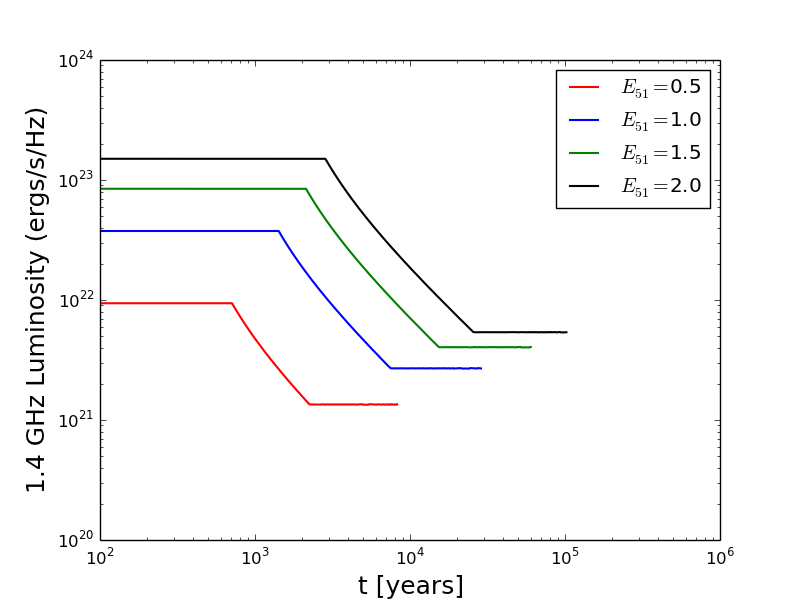
\includegraphics[width=8cm]{SNenergies.png}
		\caption{}
	\end{subfigure}
	\begin{subfigure}[b]{0.5\textwidth}
		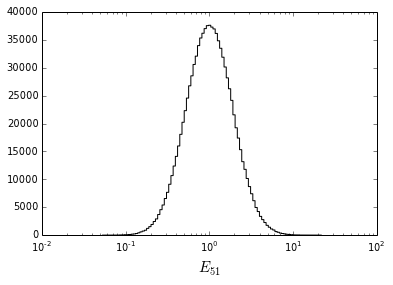
\includegraphics[width=8cm]{SNEnergydist.png}
		\caption{}
	\end{subfigure}
	\begin{subfigure}[b]{0.5\textwidth}
		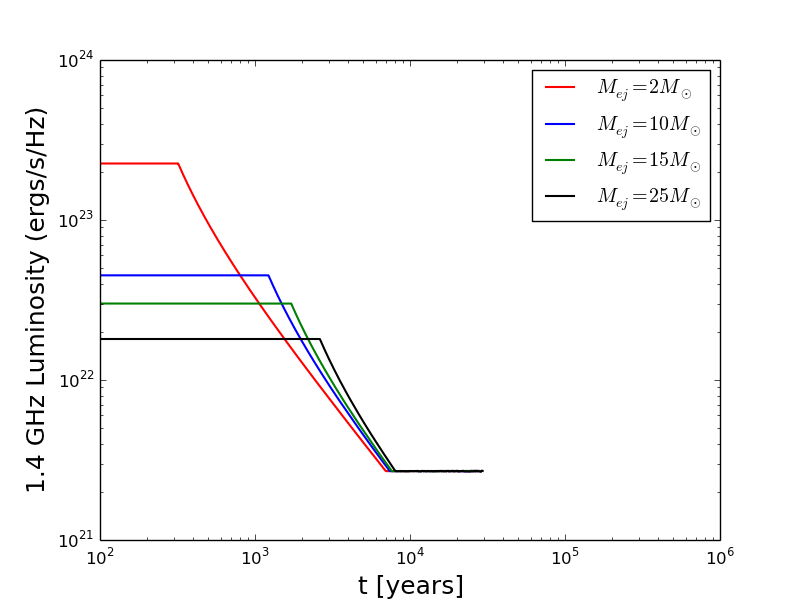
\includegraphics[width=8cm]{SNMasses.png}
		\caption{}
	\end{subfigure}
	\begin{subfigure}[b]{0.5\textwidth}
		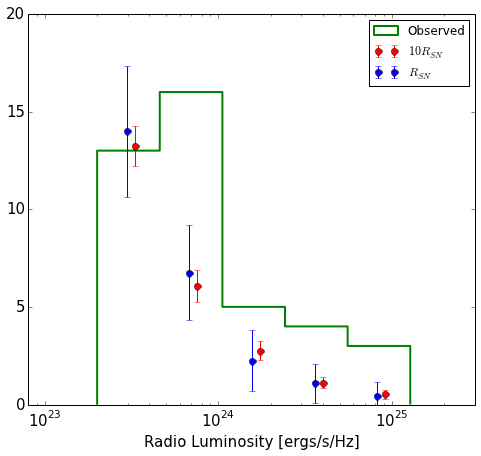
\includegraphics[width=7cm]{Likelihood.png}
		\caption{}
	\end{subfigure}
	\caption{a) Light curves for Type II SNR evolving for different $E_{51}$ at $n_0 = 1 cm^{-3}, M_{ej} = 12 M_{\odot}, \gamma = 3$. b) Log-normal distribution of $E_{51}$ centered at $10^{51}$ ergs. c) Light curves for various ejecta masses of Type II SNR growing in $n_0 = 1 cm^{-3}, E_{kin} = 1.0, \gamma = 3$. d) Likelihood estimation technique. The observed remnants are placed into 5 bins (green). The model remnants in each bin, averaged over several snapshot times, are shown with $1_\sigma$ errors, using normal $R_{SN}$, and $10 R_{SN}$, according to Jeff. As expected, Jeff's way reduces the errors in the model. All remnants are chosen at a cutoff of $2.0 \times 10^{23}$ ergs/s/Hz.}
\end{figure}
\newpage
\begin{figure}[h!]
	\begin{subfigure}[b]{0.51\textwidth}
		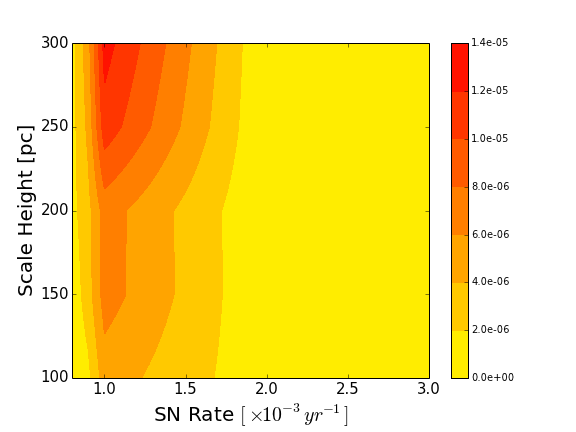
\includegraphics[width=8cm]{ScaleRate.png}
		\caption{}
	\end{subfigure}
	\begin{subfigure}[b]{0.5\textwidth}
		\includegraphics[width=8cm]{ScaleFraction.png}
		\caption{}
	\end{subfigure}
	\begin{subfigure}[b]{0.5\textwidth}
		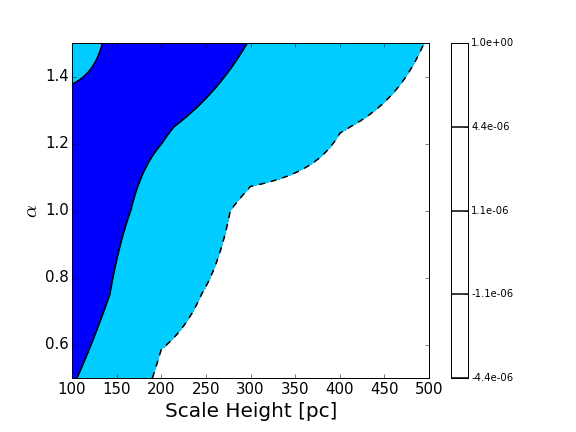
\includegraphics[width=8cm]{AlphaScale.png}
		\caption{}
	\end{subfigure}
	\begin{subfigure}[b]{0.5\textwidth}
		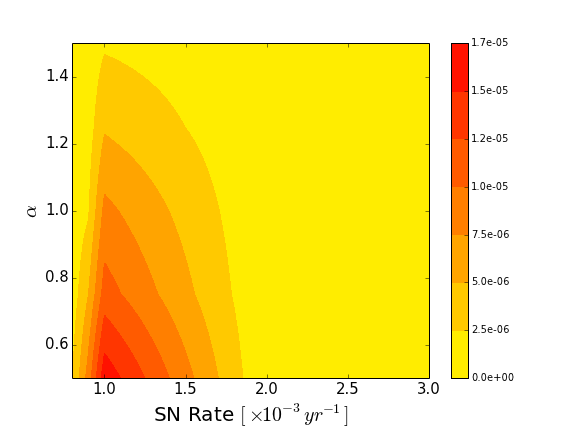
\includegraphics[width=8cm]{AlphaRate.png}
		\caption{}
	\end{subfigure}
	\begin{subfigure}[b]{0.5\textwidth}
		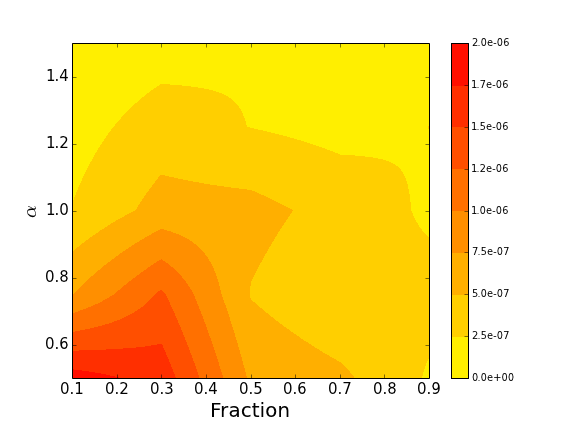
\includegraphics[width=8cm]{AlphaFraction.png}
		\caption{}
	\end{subfigure}
	\begin{subfigure}[b]{0.5\textwidth}
		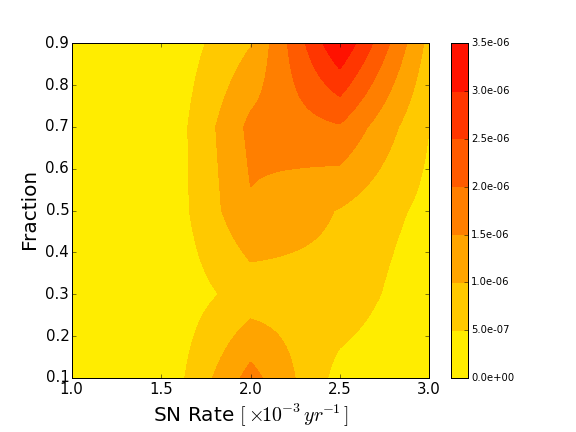
\includegraphics[width=8cm]{FractionRate.png}
		\caption{}
	\end{subfigure}
	\caption{Parameter space of our model, after marginalizing over the nuisance parameters for each plot. Here, $\gamma = 3$. Sorry I couldn't make a triangle. Will try next time.}
\end{figure}
\newpage
\begin{figure}[h!]
	\begin{subfigure}[b]{1.5\textwidth}
		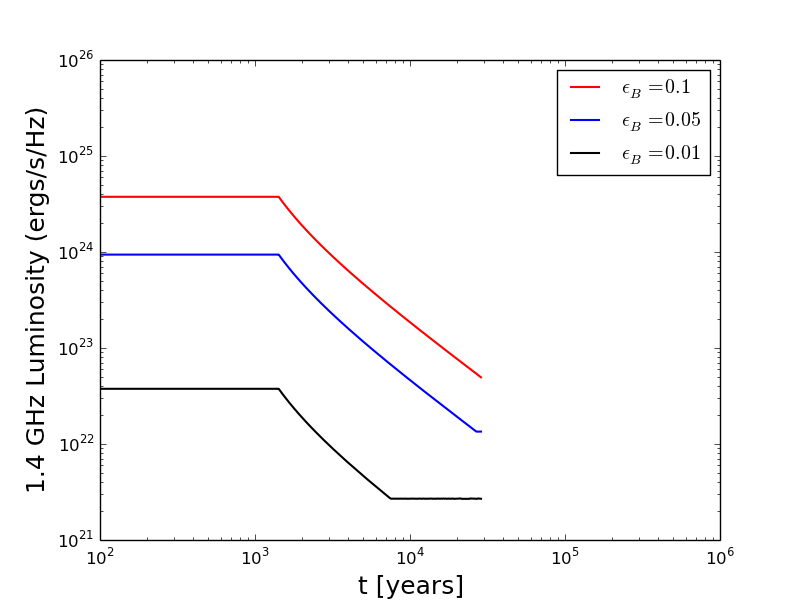
\includegraphics[width=12cm]{epsb.png}
		\caption{}
	\end{subfigure}
	\begin{subfigure}[b]{1.5\textwidth}
		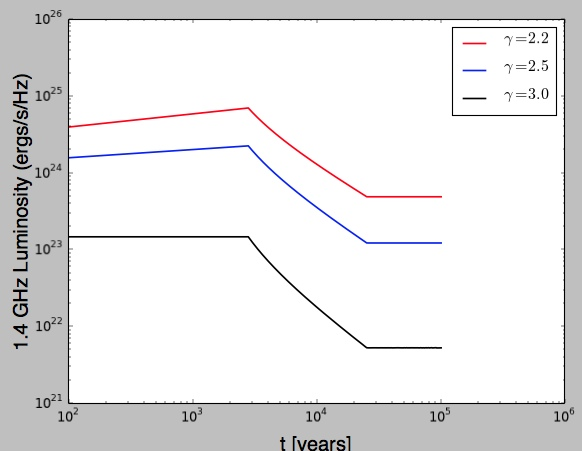
\includegraphics[width=12cm]{spectralindex.png}
		\caption{}
	\end{subfigure}
	\caption{a) Light curves of Type II SNR for different values of the equipartition fraction, $\epsilon_B$. b) Light curves for different values of the electron spectral index}
\end{figure}
\newpage
\begin{figure}[h!]
	\begin{subfigure}[b]{0.51\textwidth}
		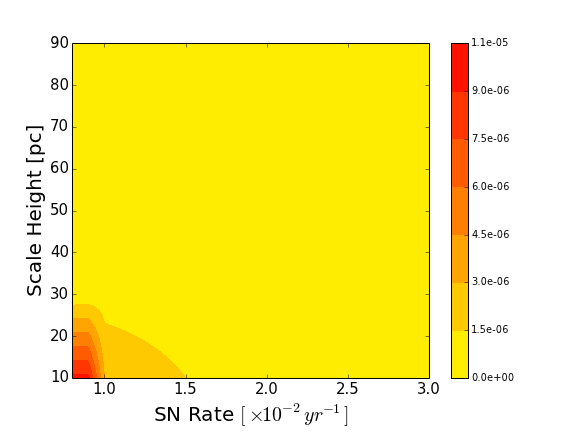
\includegraphics[width=8cm]{ScaleRate_gamma26.png}
		\caption{}
	\end{subfigure}
	\begin{subfigure}[b]{0.5\textwidth}
		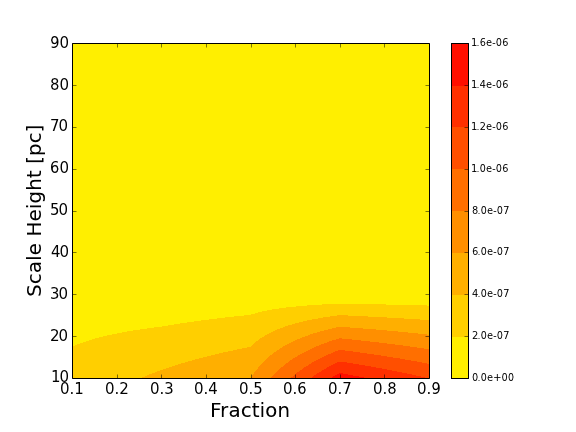
\includegraphics[width=8cm]{ScaleFraction_gamma26.png}
		\caption{}
	\end{subfigure}
	\begin{subfigure}[b]{0.5\textwidth}
		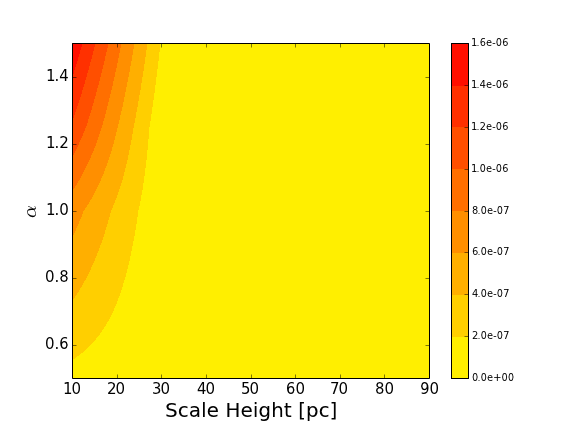
\includegraphics[width=8cm]{AlphaScale_gamma26.png}
		\caption{}
	\end{subfigure}
	\begin{subfigure}[b]{0.5\textwidth}
		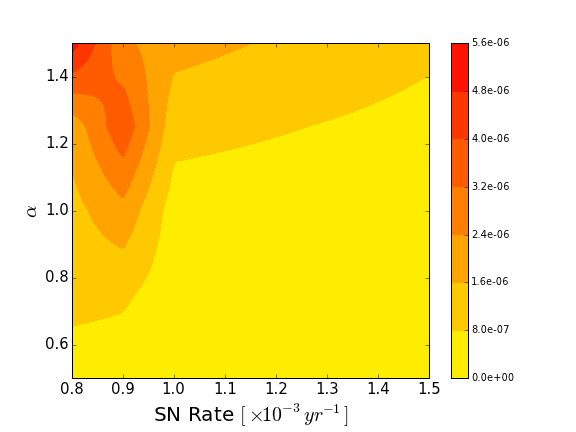
\includegraphics[width=8cm]{AlphaRate_gamma26.png}
		\caption{}
	\end{subfigure}
	\begin{subfigure}[b]{0.5\textwidth}
		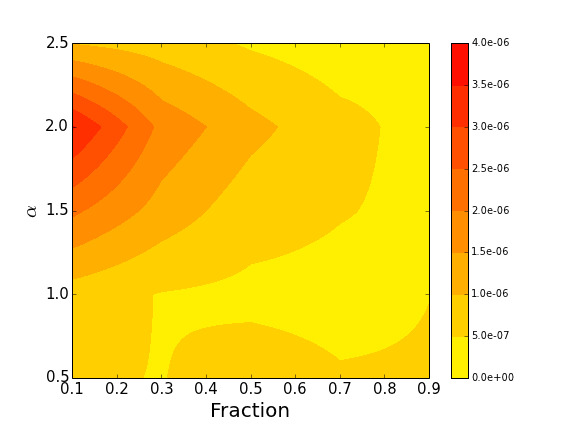
\includegraphics[width=8cm]{AlphaFraction_gamma26.png}
		\caption{}
	\end{subfigure}
	\begin{subfigure}[b]{0.5\textwidth}
		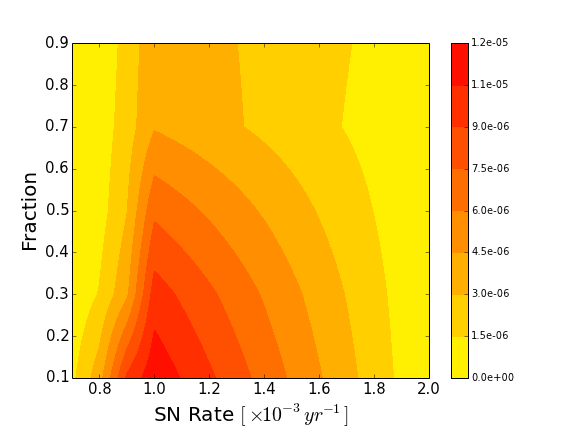
\includegraphics[width=8cm]{FractionRate_gamma26.png}
		\caption{}
	\end{subfigure}
	\caption{Parameter space of our model, after marginalizing over the nuisance parameters for each plot. Here, $\gamma = 2.6$}
\end{figure}

\end{document}